\documentclass{article}
\usepackage{amsmath}
\pagestyle{empty}
\usepackage{pgfplots}
\pgfplotsset{compat=1.9}
\raggedright
\usepackage[margin = 0.5in]{geometry}
\begin{document}

Name \makebox[3in]{\hrulefill} \hfill Hon. PreCalc P-Set   

\subsubsection*{Graphs of Sine and Cosine Functions \hfill  \makebox[0.35in]{\hrulefill} / 10} 

For each of the following, state the amplitude, period, phase shift, and vertical shift. 
\newline\\

\begin{tabular}{p{0.3\textwidth}p{0.3\textwidth}p{0.3\textwidth}}
1.     $y = 1 + 3\cos(3\theta + 135^{\circ})$		&
2. 	$y = \sin\left(\dfrac{\theta}{4} - 135^{\circ}\right) - 1$	&
3. 	$y = 2\sin(2\theta + 90^{\circ}) - 1$	\\[3.5in]
4. 		$y = 2 + 3\cos\dfrac{\theta}{4}$	&
5. 		$y = \dfrac{1}{2}\cos\left(2\theta - \dfrac{\pi}{2}\right) - 2$	&
6. 		$y = -2 + 4\cos\left(2\theta - \frac{3\pi}{4}\right)$	\\
\end{tabular}

\newpage


Find the equation of each in the form $y = a\sin(bx)$.
\newline\\

\begin{tabular}{p{0.5\linewidth}p{0.5\linewidth}}
7.		&	8. 	\\[0.25in]
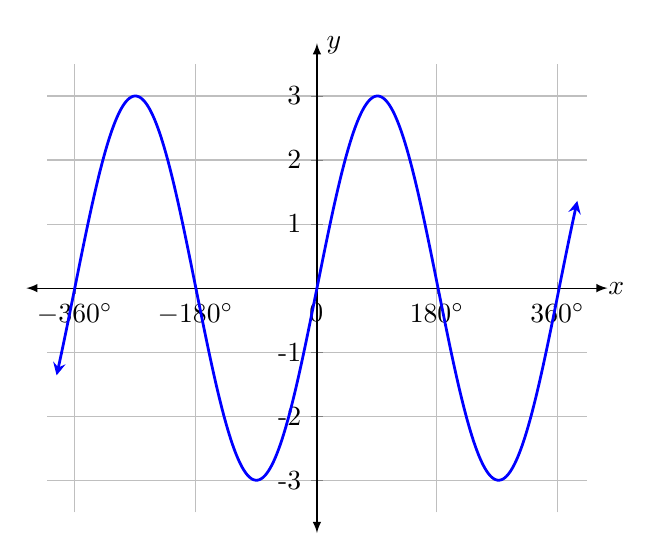
\begin{tikzpicture}
\begin{axis}
[   
    grid,
    axis lines=middle,
    xmin=-7,xmax=7,
    ymin=-3.5,ymax=3.5,
    restrict y to domain=-3.5:3.5,
    xtick={-6.28318, -3.15159265, ..., 6.28318},
    xticklabels={$-360^\circ$,$-180^\circ$,0,$180^\circ$,$360^\circ$},
    ytick={-3,-2,...,5},
    yticklabels={-3,-2,-1,,1,2,3,4,5},
    axis line style={latex-latex},
    axis line style={shorten >=-7.5pt, shorten <=-7.5pt},
    xlabel=$x$,
    ylabel=$y$,
    xlabel style={at={(ticklabel* cs:1)},anchor=west, xshift=0.15cm},
    ylabel style={at={(ticklabel* cs:1)},anchor=south west}
]
\addplot+[no marks, domain=-2.15*pi:2.15*pi, samples=500,<->, > = stealth, line width = 1]{3*sin(deg(x))};
\end{axis}

\end{tikzpicture}
&
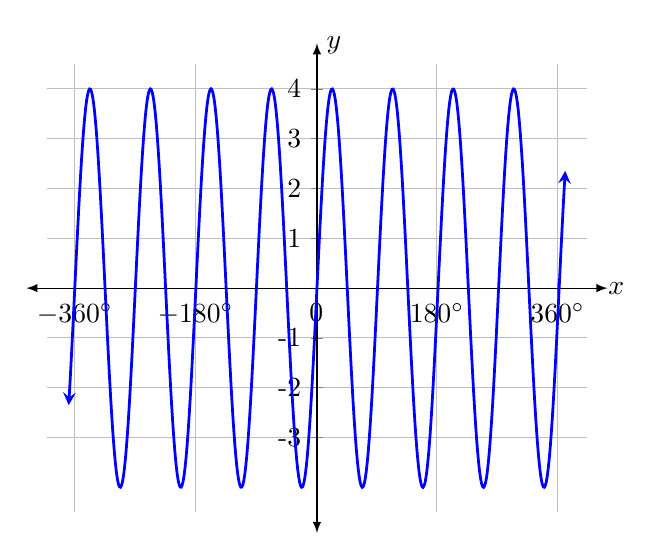
\begin{tikzpicture}
\begin{axis}
[   
    grid,
    axis lines=middle,
    xmin=-7,xmax=7,
    ymin=-4.5,ymax=4.5,
    restrict y to domain=-4.5:4.5,
    xtick={-6.28318, -3.15159265, ..., 6.28318},
    xticklabels={$-360^\circ$,$-180^\circ$,0,$180^\circ$,$360^\circ$},
    ytick={-3,-2,...,5},
    yticklabels={-3,-2,-1,,1,2,3,4,5},
    axis line style={latex-latex},
    axis line style={shorten >=-7.5pt, shorten <=-7.5pt},
    xlabel=$x$,
    ylabel=$y$,
    xlabel style={at={(ticklabel* cs:1)},anchor=west, xshift=0.15cm},
    ylabel style={at={(ticklabel* cs:1)},anchor=south west}
]
\addplot+[no marks, domain=-2.05*pi:2.05*pi, samples=500,<->, > = stealth, line width = 1]{4*sin(deg(4*x))};
\end{axis}
\end{tikzpicture}
\\[0.5in]	
9. 		&	10. 	\\[0.25in]
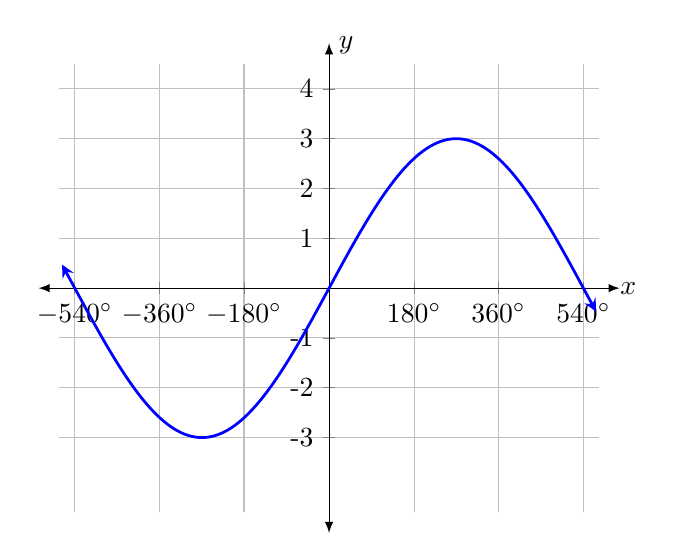
\begin{tikzpicture}
\begin{axis}
[   
    grid,
    axis lines=middle,
    xmin=-10,xmax=10,
    ymin=-4.5,ymax=4.5,
    restrict y to domain=-4.5:4.5,
    xtick={-9.42477796, -6.28318, -3.15159265, 0, 3.15159265,6.28318 , 9.42477796},
    xticklabels={$-540^\circ$, $-360^\circ$,$-180^\circ$,0,$180^\circ$,$360^\circ$, $540^\circ$},
    ytick={-3,-2,...,5},
    yticklabels={-3,-2,-1,,1,2,3,4,5},
    axis line style={latex-latex},
    axis line style={shorten >=-7.5pt, shorten <=-7.5pt},
    xlabel=$x$,
    ylabel=$y$,
    xlabel style={at={(ticklabel* cs:1)},anchor=west, xshift=0.15cm},
    ylabel style={at={(ticklabel* cs:1)},anchor=south west}
]
\addplot+[no marks, domain=-3.15*pi:3.15*pi, samples=500,<->, > = stealth, line width = 1]{3*sin(deg(x/3))};
\end{axis}
\end{tikzpicture}
&
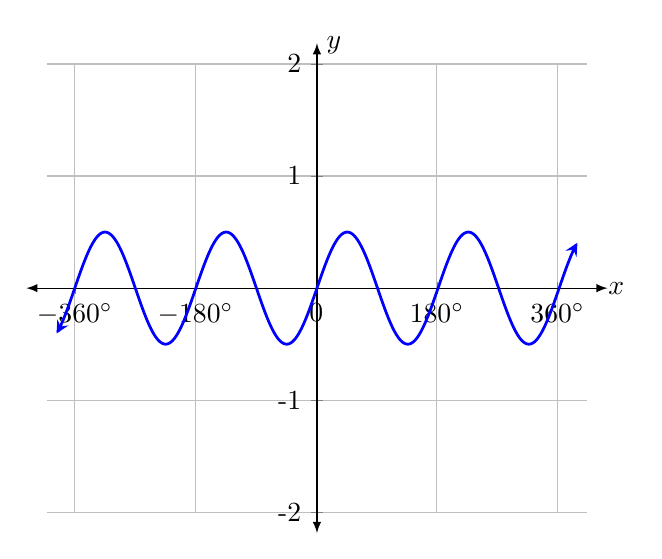
\begin{tikzpicture}
\begin{axis}
[   
    grid,
    axis lines=middle,
    xmin=-7,xmax=7,
    ymin=-2,ymax=2,
    restrict y to domain=-2:2,
    xtick={-6.28318, -3.15159265, ..., 6.28318},
    xticklabels={$-360^\circ$,$-180^\circ$,0,$180^\circ$,$360^\circ$},
    ytick={-2,-1,...,2},
    yticklabels={-2,-1,...,2},
    axis line style={latex-latex},
    axis line style={shorten >=-7.5pt, shorten <=-7.5pt},
    xlabel=$x$,
    ylabel=$y$,
    xlabel style={at={(ticklabel* cs:1)},anchor=west, xshift=0.15cm},
    ylabel style={at={(ticklabel* cs:1)},anchor=south west}
]
\addplot+[no marks, domain=-2.15*pi:2.15*pi, samples=500,<->, > = stealth, line width = 1]{0.5*sin(deg(2*x))};
\end{axis}
\end{tikzpicture}
\end{tabular}
\bigskip


11. The functions $f(x) = \frac{\sin x}{x}$ and $g(x) = \frac{1 - \cos x}{x}$ are not defined when $x = 0$ (note that $x$ is in radians).
\newline\\


Use a calculator to approximate values of $f(x)$ and $g(x)$ near $x = 0$, such as $x = \pm 0.01$, $x = \pm 0.001$, etc.
\newline\\


What value(s) do $f(x)$ and $g(x)$ appear to approach as $x$ gets closer and closer to 0?



\newpage


\textbf{Graphs of Sine and Cosine Functions KEY}

\begin{enumerate}
    \item Amp = 3, Per = $120^\circ$, P.S. = $45^\circ$ left, V.S. = up 1
    
    \item Amp = 1, Per = $1440^\circ$, P.S. = $540^\circ$ right, V.S. = down 1
    
    \item Amp = 2, Per = $180^\circ$, P.S. = $45^\circ$ left, V.S. = down 1
    
    \item Amp = 3, Per = $1440^\circ$, P.S. = None, V.S. = up 2
    
    \item Amp = $\frac{1}{2}$, Per = $\pi$, P.S. = $\frac{\pi}{4}$ left, V.S. = down 2
    
    \item Amp = 4, Per = $\pi$, P.S. = $\frac{3\pi}{8}$ right, V.S. = down 2
    
    \item $y = 3\sin x$
    
    \item $y = 4\sin 4x$
    
    \item $y = 3\sin\left(\frac{x}{3}\right)$
    
    \item $y = \frac{1}{2}\sin 2x$
\end{enumerate}



\end{document}
